\documentclass[sigconf]{acmart}

\setcopyright{none}
\acmConference[G67]{PRI}{October 2026}{Porto, Portugal}
\renewcommand\footnotetextcopyrightpermission[1]{}

\begin{document}

\title{GRIDLY: SEARCHING THE HISTORY OF FORMULA 1}

\author{Emilie Kernivinen}
\email{up202306154@up.pt}
\affiliation{%
  \institution{Faculty of Engineering - University of Porto}
  \city{Porto}
  \country{Portugal}}

\author{João Marques}
\email{up202307612@up.pt}
\affiliation{%
  \institution{Faculty of Engineering - University of Porto}
  \city{Porto}
  \country{Portugal}}

\author{João Ferreira}
\email{up202305204@up.pt}
\affiliation{%
  \institution{Faculty of Engineering - University of Porto}
  \city{Porto}
  \country{Portugal}}

\author{José Ferreira}
\email{up202305478@up.pt}
\affiliation{%
  \institution{Faculty of Engineering - University of Porto}
  \city{Porto}
  \country{Portugal}}

\renewcommand{\shortauthors}{Emilie Kernivinen, João Marques, João Ferreira and José Ferreira}

\renewcommand{\abstractname}{ABSTRACT}
\begin{abstract}
  Information about Formula One is spread across numerous sources, so fans who want to explore the history of the sport have to combine several of them. This project addresses this need by building a search system that brings Formula One data together in a single place.

  We combine structured data from the Jolpica F1 database, which provides race results and championship
  records, with text from English Wikipedia articles, linking each record to its article covering the 1950 to 2026 seasons.
\end{abstract}


\begin{CCSXML}
<ccs2012>
<concept>
<concept_id>10002951.10003317.10003325</concept_id>
<concept_desc>Information systems~Information retrieval query processing</concept_desc>
<concept_significance>100</concept_significance>
</concept>
</ccs2012>
\end{CCSXML}

\ccsdesc[100]{Information systems~Information retrieval query processing}

\keywords{Formula One, Motorsport, Information Retrieval, Search System,
  Wikipedia, Jolpica F1, Data Preparation, Data Quality, Conceptual Model,
  Collection Characterization}


\begin{teaserfigure}
  \includegraphics[width=\textwidth]{imgs/f1_primordials.png}
  \caption{Farina leads Fagioli at the 1950 British Grand Prix, the first Formula One World Championship race. Image via Gasolina na Veia (\url{https://gasolinanaveia.com.br}).}
  \Description{Two vintage racing cars on a track lined with straw bales.}
  \label{fig:teaser}
\end{teaserfigure}

\maketitle


% =====================================================================
\section{Introduction}
This work was developed for the course ``Information Processing and
Retrieval'' (PRI) of the Master's in Informatics and Computing Engineering
(M.EIC) at the Faculty of Engineering of the University of Porto (FEUP).

The choice of Formula One is motivated both by personal interest and by the
nature of its data. Most of us follow the sport, but as relatively recent
fans we wanted an easy way to learn about its history, which goes back to
the first World Championship race in 1950. This history comes in two forms:
structured data, such as results and championship standings, and free text,
such as race reports and driver biographies. Many questions need both. For
example, finding races decided by a late mechanical failure requires
matching the retirement reason in the results with the narrative of the
race, which makes Formula One a good domain for an information retrieval
system close to a real-world scenario.

This report covers Milestone 1, whose goal is to build the document
collection. Section~\ref{sec:dataset} describes the dataset, from its
sources and preparation to its quality, structure and characterization.
Section~\ref{sec:needs} presents the search scenarios, and
Section~\ref{sec:conclusions} concludes and outlines the next milestone.

% =====================================================================
\section{Dataset}
\label{sec:dataset}

\subsection{Data Origin and Description}
\label{sec:sources}
Two complementary sources were selected, as they cover the full history of
the sport: the Jolpica F1 database and the English Wikipedia.
Table~\ref{tab:sources} characterizes both as downloaded. For Jolpica,
rows and columns are summed over its 11 tables; for Wikipedia, each row is
an article and the columns are the fields stored for it.

\begin{table}[h]
  \small
  \caption{Initial data sources characterization}
  \label{tab:sources}
  \begin{tabular}{llrrrr}
    \toprule
    Source & Format & Files & Rows & Columns & Size (MB) \\
    \midrule
    Jolpica F1 & CSV & 11 & 141029 & 110 & 7.30 \\
    Wikipedia (EN) & JSON & 2225 & 2225 & 7 & 77.37 \\
    \bottomrule
  \end{tabular}
\end{table}

Jolpica F1~\cite{jolpica} is an open-source project that succeeds the Ergast
API, discontinued at the end of 2024. Its relational database holds the
results of every World Championship race since 1950, including starting
grids, finishing positions, retirement reasons, team line-ups and
championship standings. We used its CSV dump instead of the REST API, which
would require around 260 paginated requests under an hourly rate limit.
Wikipedia~\cite{wikipedia} provides the text: the narrative of each race,
the biography of each driver and the history of each team and circuit. The
articles were obtained in wikitext through the MediaWiki Action
API~\cite{mediawikiapi}, which returns several articles per request.

The two sources are linked by Jolpica itself, which stores the Wikipedia
URL of every race, driver, team and circuit. This avoids matching by name,
which would be error-prone for drivers with the same name or races whose
title changed over the years. Both sources have public licenses (CC
BY-NC-SA 4.0 for Jolpica and CC BY-SA 4.0 for Wikipedia) that allow their
use in an academic project.

\subsection{Data Preparation}
\label{sec:pipeline}
The pipeline (Figure~\ref{fig:pipeline}) is implemented in Python as five
scripts, each reading the output of the previous one. Raw downloads,
intermediate files and the final collection are kept in separate folders.

\textbf{Collection.} The first script downloads the Jolpica dump, keeps the
11 tables needed and records the version used (12 September 2026), since
the dump link always points to the latest one. The third script downloads
the Wikipedia article linked to each record. Since Wikipedia blocks
anonymous clients that send one request per page (HTTP 429), articles are
requested in batches of 20, reducing about 2230 requests to 115. Each
article is cached locally with its page and revision identifiers, which
identify the exact version used.

\textbf{Processing.} The second script joins the Jolpica tables with
Pandas~\cite{pandas} into one record per race, driver, team and circuit,
with values such as the winner and retirements of a race or the career
totals of a driver. Jolpica has one team row per chassis--engine combination
(``Cooper-Climax'', ``Cooper-Maserati''), so rows that point to the same
article were merged into one team. Only races already held were kept. The
totals were checked against known facts, such as Ayrton Senna's 41 wins.
The fourth script converts the wikitext to clean text with
mwparserfromhell~\cite{mwparserfromhell}: tables, references, infoboxes,
images and categories are removed, links are replaced by their visible text,
and templates that are part of a sentence, such as unit conversions, keep
their text. Each article is then split by its sections, which are mapped by
keywords to a fixed set of text fields per document type
(Table~\ref{tab:fields}). For example, a race section called ``Race
report'' goes to the \texttt{race} field, while sections without prose,
such as the classification tables or the championship standings, are
discarded. Having fixed fields will allow each part of a document to be
weighted differently in the next milestone. Finally, documents with less
than 100 words of text are rejected, with the reason recorded.

\textbf{Chaining.} Each structured record is joined to its article through
the Jolpica link, and the documents are linked to each other in both
directions (races, drivers and teams, and races and circuits), keeping only
links between accepted documents. The result is exported in JSON and CSV.
The fifth script computes the statistics and plots of
Section~\ref{sec:characterization}, using Matplotlib~\cite{matplotlib},
NumPy~\cite{numpy} and scikit-learn~\cite{scikitlearn}.

\textbf{Makefile.} The whole pipeline runs with \texttt{make}, which creates
the virtual environment, installs the dependencies and runs the five steps
in order. Each step has its own target (\texttt{collect},
\texttt{structure}, \texttt{wikipedia}, \texttt{documents},
\texttt{analyze}), \texttt{make clean} removes the generated files but keeps
the downloads, and \texttt{make clean-all} removes everything.

\begin{figure}[h]
  \centering
  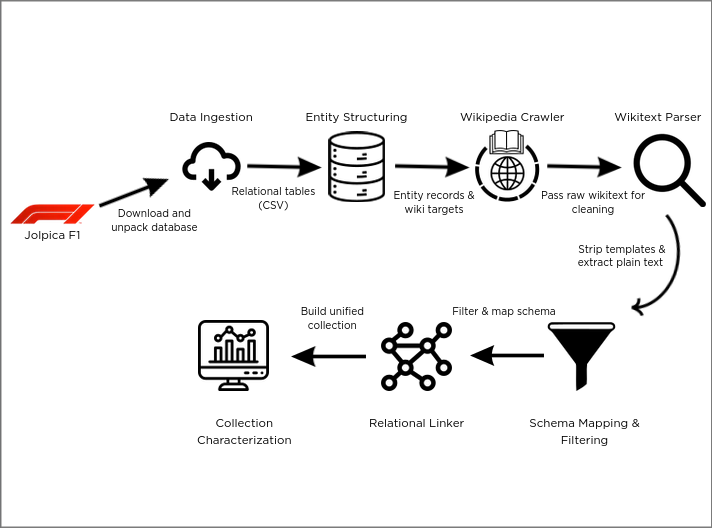
\includegraphics[width=\linewidth]{imgs/pipeline.png}
  \caption{Data preparation pipeline}
  \Description{Diagram of the five pipeline steps. The Jolpica F1 CSV dump is
  collected and joined into structured records of races, drivers, teams and
  circuits. Their Wikipedia links are used to download the articles, which are
  combined with the structured records into the final JSON and CSV collection,
  which is then analyzed to produce statistics and plots.}
  \label{fig:pipeline}
\end{figure}

\subsection{Data Quality}
\label{sec:quality}
Table~\ref{tab:quality} lists the problems found and how they were handled.
Most come from the links between the sources. In 28 cases, the Jolpica link
leads to a \textbf{disambiguation page} (``Tony Brooks may refer
to\ldots''), usually because a more famous person has the same name.
Fixing these by hand would not survive a new run of the pipeline, so they
are resolved automatically: the script prefers the entry whose title
mentions ``Formula One'' or ``racing driver'', then one on a line that
mentions Formula One, and finally one on a line that mentions racing. For
example, ``Tony Brooks'' becomes ``Tony Brooks (racing driver)'', and each
correction is recorded with the original link. The Long Beach circuit links
to the article about the city, which is a valid article and cannot be
detected automatically, so it was corrected by hand.

In the results, the \textbf{status} is a numeric code with no
documentation. By grouping the values of the \texttt{detail} column
(``Engine'', ``Spun off'', ``+1 Lap'') under each code, we inferred its
meaning: finished, finished with laps behind, retired by accident, retired
by failure, disqualified and did not start. This made it possible to keep
the retirement reasons, one of the most useful structured fields.

Most of the 164 \textbf{short documents} are drivers from the 1950s with one
or two races, whose article is a single sentence followed by a table. The
threshold was chosen by looking at these articles: with 150 words, 111 more
documents would be lost, many of them with useful text. One side effect is
that the Pedralbes circuit was rejected, so its two races have no linked
circuit document.

\begin{table}[h]
  \small
  \caption{Data quality issues and how they were handled}
  \label{tab:quality}
  \begin{tabular}{p{3.6cm}rp{2.8cm}}
    \toprule
    Issue & Count & Handling \\
    \midrule
    Links to disambiguation pages & 28 & resolved automatically \\
    Link to the wrong article (Long Beach) & 1 & fixed manually \\
    Links to missing articles & 3 & rejected \\
    Documents under 100 words & 164 & rejected \\
    Team rows sharing one article & 40 & merged \\
    Undocumented numeric \texttt{status} & -- & inferred from \texttt{detail} \\
    HTML entities in names & 1 & decoded \\
    \bottomrule
  \end{tabular}
\end{table}

\subsection{Final Dataset}
\label{sec:final}
The final collection has 2058 documents of four types
(Table~\ref{tab:collection}). Each document combines structured fields from
Jolpica, useful for filters, with text fields from Wikipedia, which are the
ones searched (Table~\ref{tab:fields}). All documents also keep the article
URL and revision and their word count.

\begin{table}[h]
  \small
  \caption{Final collection}
  \label{tab:collection}
  \begin{tabular}{lrrrrr}
    \toprule
     & Races & Drivers & Teams & Circuits & Total \\
    \midrule
    Jolpica records & 1162 & 818 & 168 & 77 & 2225 \\
    Accepted & 1116 & 719 & 147 & 76 & 2058 \\
    Rejected & 46 & 99 & 21 & 1 & 167 \\
    Median words & 827 & 690 & 1082 & 1238 & -- \\
    \bottomrule
  \end{tabular}
\end{table}

\begin{table}[h]
  \small
  \caption{Main fields of each document type}
  \label{tab:fields}
  \begin{tabular}{p{1.1cm}p{4.0cm}p{2.3cm}}
    \toprule
    Type & Structured fields & Text fields \\
    \midrule
    Race & season, date, circuit, country, winner, pole, podium, fastest
    lap, starters, finishers, retirements & summary, background,
    qualifying, race, post\_race \\
    Driver & nationality, birth date, seasons, teams, wins, podiums, poles,
    championships & summary, biography \\
    Team & names, nationality, seasons, wins, podiums, championships &
    summary, history \\
    Circuit & locality, country, coordinates, Grands Prix, most wins &
    summary, history, layout, events \\
    \bottomrule
  \end{tabular}
\end{table}

\subsection{Conceptual Model}
\label{sec:model}
The conceptual model (Figure~\ref{fig:model}) has four entities, matching
the document types. A driver takes part in one or more races and each race
has several drivers; this relation holds the grid position, finishing
position and status. A driver drives for one or more teams, and a team has
at least one driver, not necessarily two: 47 Jolpica teams had a single
driver in their whole history, mostly private entries of the 1950s. A race
has one or more teams, and each race is held at exactly one circuit. In the
JSON documents, relations are stored as lists of identifiers in both
directions (e.g., \texttt{driver\_ids} in a race and \texttt{race\_ids} in a
driver).

\begin{figure}[h]
  \centering
  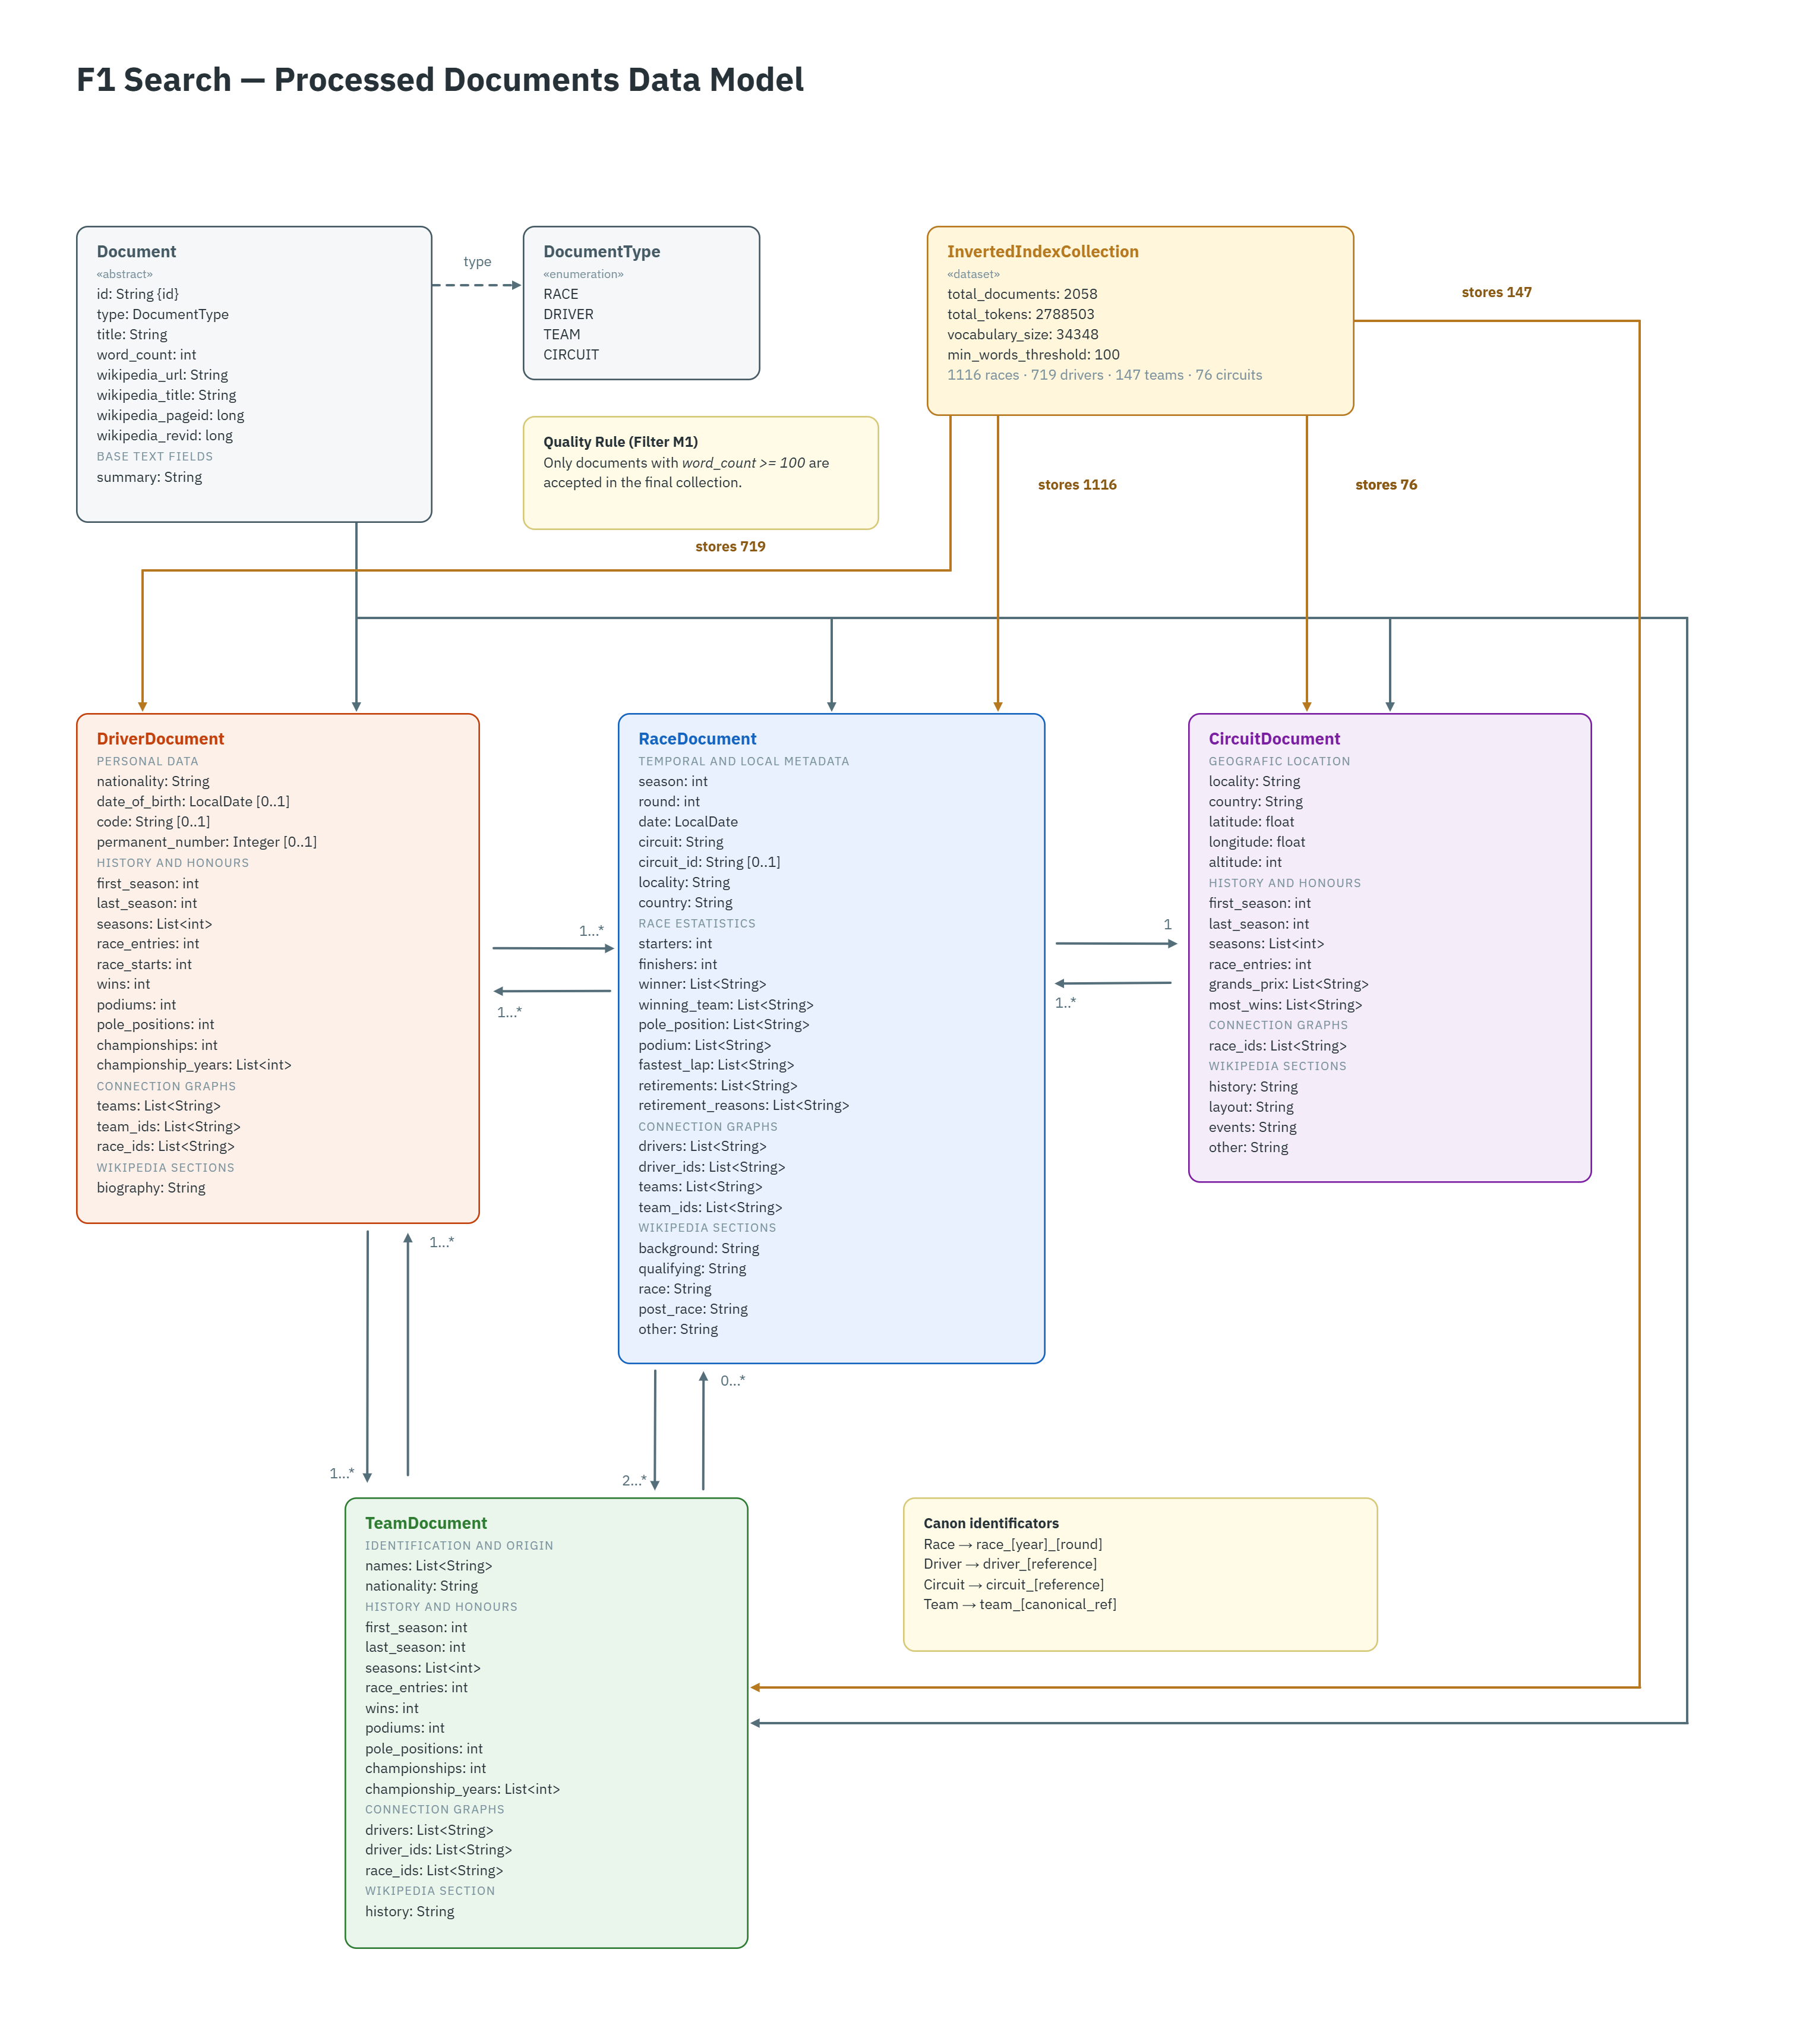
\includegraphics[width=\linewidth]{imgs/conceptual_model.png}
  \caption{Domain conceptual model}
  \Description{UML class diagram with four classes: Driver, Race, Team and
  Circuit. Driver and Race are linked by a many-to-many association with
  grid, position and status. Driver and Team, and Race and Team, are also
  many-to-many. Race is linked to exactly one Circuit, and a Circuit to one
  or more Races.}
  \label{fig:model}
\end{figure}

\subsection{Data Characterization}
\label{sec:characterization}
Document length is very uneven (Figure~\ref{fig:wordcount}). In every type
the mean is well above the median, pulled up by a few long articles: the
longest driver document (Kimi Räikkönen) has 14454 words, twenty times the
median. For races, length depends on the period
(Figure~\ref{fig:decade}): the median goes from about 330 words in the 1960s
to 1849 in the 2000s, almost six times more. The 2000s are the peak, which
suggests that these seasons were written about as they happened by a large
community of editors, while older races were documented later and with
fewer sources. This matters for the search system: a long document has more
chances of matching a query, so a ranking that does not normalize length
well will tend to favor recent races.

\begin{figure*}[t]
  \centering
  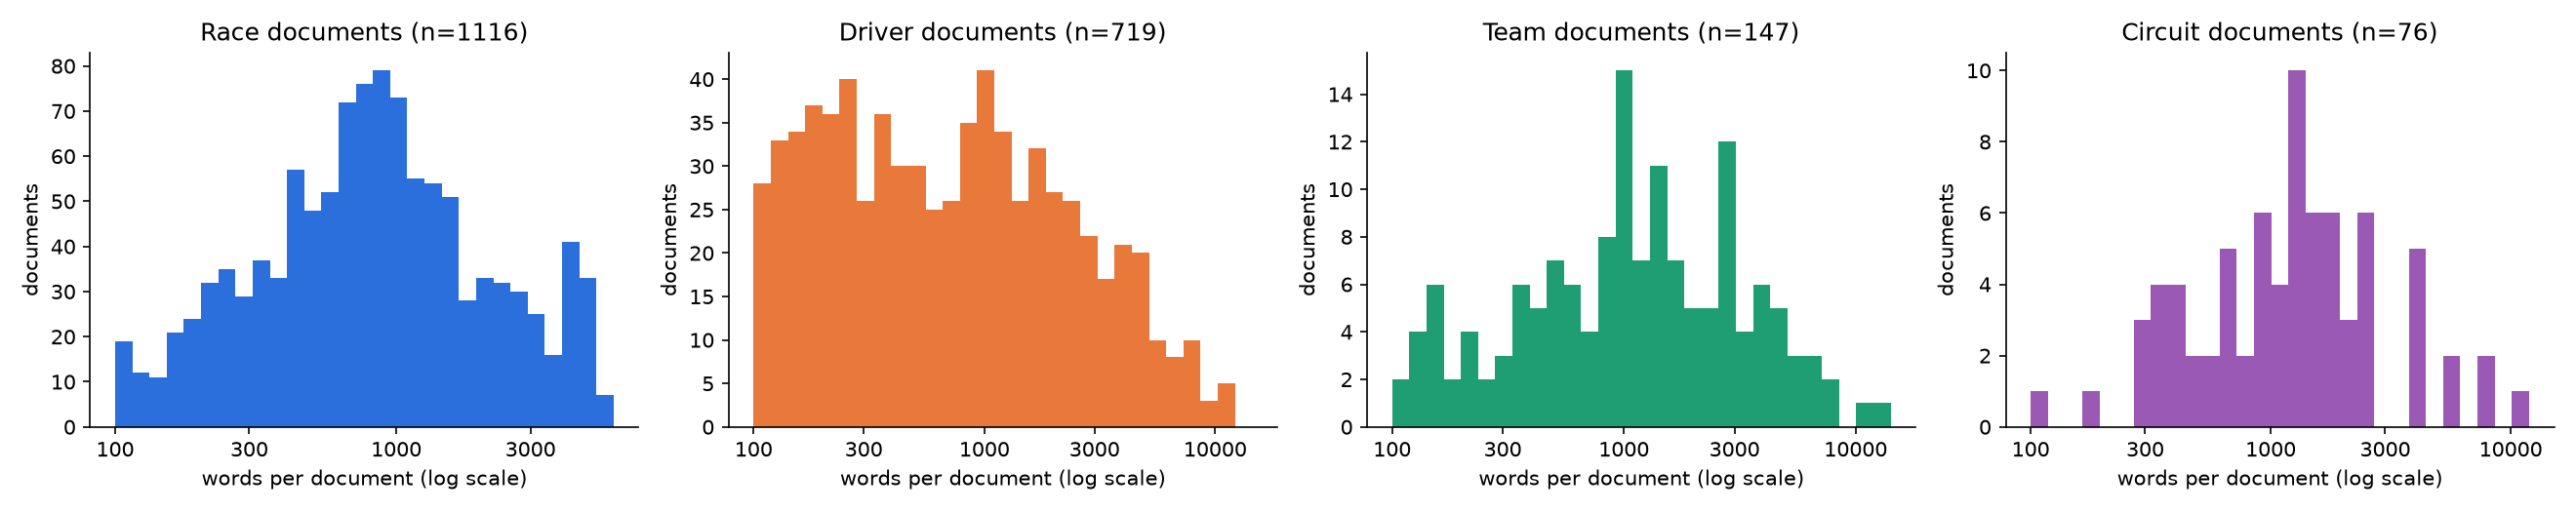
\includegraphics[width=\textwidth]{imgs/word_count_distribution.png}
  \caption{Words per document, by document type (log scale)}
  \Description{Four histograms, one per document type, with words per
  document on a logarithmic axis from 100 to over 10000. Race documents peak
  around 1000 words; driver documents are spread evenly between 100 and 3000
  words; team and circuit documents are fewer and peak around 1000 words.}
  \label{fig:wordcount}
\end{figure*}

The collection has 2.79 million tokens and a vocabulary of 34348 terms,
37\% of which appear only once, mostly uncommon words and names of people
and places mentioned in a single article. Stopwords make up 45\% of all
tokens. Term frequency follows Zipf's law~\cite{manning2008} between ranks
10 and about 2000 (Figure~\ref{fig:zipf}), with the usual deviations at both
ends: the most frequent words are less frequent than the law predicts, and
the tail falls faster. The vocabulary grows sublinearly, as Heaps' law
predicts (Figure~\ref{fig:heaps}). Since documents are read grouped by type,
the curve also shows a difference between them: the growth almost stops
during the race documents, which reuse the names and terms already seen in
the biographies, and rises again with the teams, which bring company names
and technical vocabulary.

After removing stopwords, ``championship'', ``prix'', ``race'' and
``formula'' appear in about 95\% of the documents, so they will have little
weight in a ranking based on inverse document frequency. The terms specific
to each type are more telling (Figure~\ref{fig:topterms}): races use
``lap'', ``pit'', ``qualifying'' and ``tyres'', teams ``engine'', and
circuits ``track'' and ``turn''. In the structured fields, engine failures
are the most common retirement reason (1889 cases), but accidents,
collisions and spins together exceed 2500 (Figure~\ref{fig:retirements}).
British (142) and American (131) drivers are the most common
(Figure~\ref{fig:nationalities}); the high number of Americans comes from
the Indianapolis 500, which counted for the championship from 1950 to 1960
and brought many drivers who never raced in Europe. Finally, every race has
a summary and 85\% have a race report, but only 42\% describe qualifying
and 27\% the aftermath (Figure~\ref{fig:coverage}), so some queries can only
be answered for part of the collection, mostly recent seasons.

% =====================================================================
\section{Search Scenarios}
\label{sec:needs}
Table~\ref{tab:needs} lists the information needs that will be used to
evaluate the system. They were chosen so that they depend on the text and
not only on the structured fields, cover three document types, can be
expressed with varied vocabulary, and have answers in the collection, which
we confirmed by finding relevant documents for each. For each need we
defined what makes a document relevant and what does not. In N2, for
example, a race is relevant only if it was affected by rain \textbf{and}
had an unusual result, such as the 1975 Austrian Grand Prix, won by Vittorio
Brambilla in a March, or the 1996 Monaco Grand Prix, where only three cars
finished. A wet race won by the favorite is not relevant.

\begin{table}[h]
  \small
  \caption{Information needs}
  \label{tab:needs}
  \begin{tabular}{lp{5.4cm}l}
    \toprule
    ID & Information need & Type \\
    \midrule
    N1 & Races decided by a pit-stop or tyre strategy & race \\
    N2 & Wet races with a surprising result & race \\
    N3 & Safety car periods that changed the result & race \\
    N4 & Collisions between teammates & race \\
    N5 & Race weekends with a fatal accident & race \\
    N6 & Disqualifications for technical infringements & race \\
    N7 & Drivers who returned after a serious injury & driver \\
    N8 & Drivers who succeeded at Le Mans or Indianapolis & driver \\
    N9 & Teams that collapsed for financial reasons & team \\
    N10 & Technical innovations that were later banned & team \\
    \bottomrule
  \end{tabular}
\end{table}

Some needs are hard on purpose. In N1, the same idea appears as
``undercut'', ``two-stop strategy'' or ``gambled on not needing a pit
stop''; in N4, the text often gives only the two names, so the
\texttt{teams} field is needed; N7 has few documents that use the words of
the query, even though there are well-known cases such as Niki Lauda or
Felipe Massa; and in N10, ``banned'' mostly returns the ban on turbo
engines, which affected every team and is not relevant. These cases will
show the limits of a search based only on words and are a good starting
point for the comparison with semantic search in the third milestone.

% =====================================================================
\section{Conclusions and Future Work}
\label{sec:conclusions}
In this milestone we built a collection of 2058 documents about the history
of Formula One, combining Jolpica F1 results with Wikipedia text through a
reproducible pipeline that runs with a single command and records the
versions of the data it used. We also analyzed the collection and defined
ten information needs.

The hardest part was the text. Wikipedia limits anonymous requests, which
forced us to download the articles in batches, and the wikitext needed a
fair amount of cleaning, since it mixes prose with tables, templates and
references. The disambiguation pages were also a problem we did not expect,
since the links came from a source we trusted. The amount of text also
varies a lot with the period, which will have to be considered when
ranking.

In the next milestone, the collection will be indexed in Apache
Solr~\cite{solr}. As the text is already split into fields, we will compare
a simple setup with one that weights the most relevant fields and uses the
structured fields as filters, evaluating both with the information needs
above through precision at $k$ and mean average precision.

% =====================================================================
\bibliographystyle{ACM-Reference-Format}
\bibliography{references}

\appendix

\section{Additional Figures}

\begin{figure}[h]
  \centering
  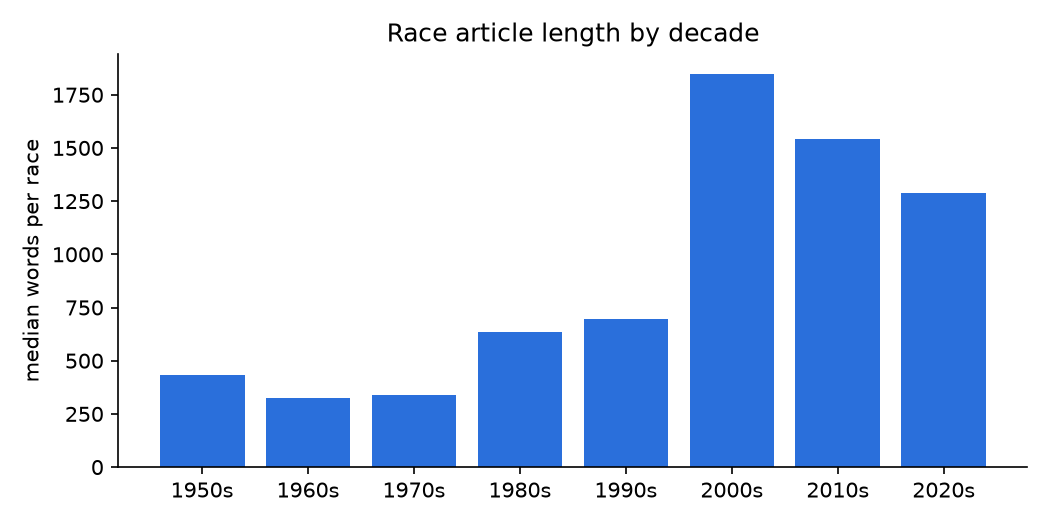
\includegraphics[width=\linewidth]{imgs/race_words_by_decade.png}
  \caption{Median words per race document, by decade}
  \Description{Bar chart of median words per race from the 1950s to the
  2020s. The values stay between about 320 and 430 until the 1970s, rise to
  about 650 to 700 in the 1980s and 1990s, peak at about 1850 in the 2000s
  and then decrease to about 1540 and 1290.}
  \label{fig:decade}
\end{figure}

\begin{figure}[h]
  \centering
  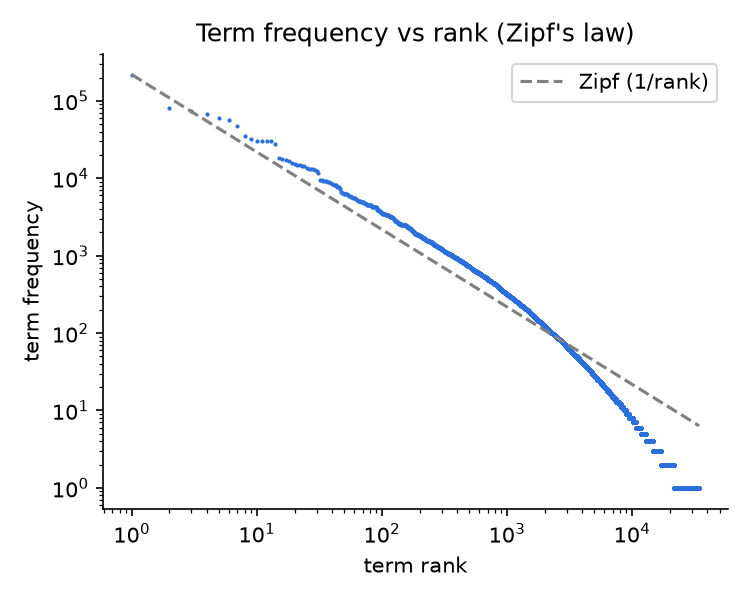
\includegraphics[width=\linewidth]{imgs/zipf.png}
  \caption{Term frequency versus rank}
  \Description{Log-log plot of term frequency against term rank. The points
  follow a dashed reference line of slope minus one for most of the range,
  lie above it for ranks 10 to 2000 and fall below it after rank 3000,
  ending in a flat line at frequency one.}
  \label{fig:zipf}
\end{figure}

\begin{figure}[h]
  \centering
  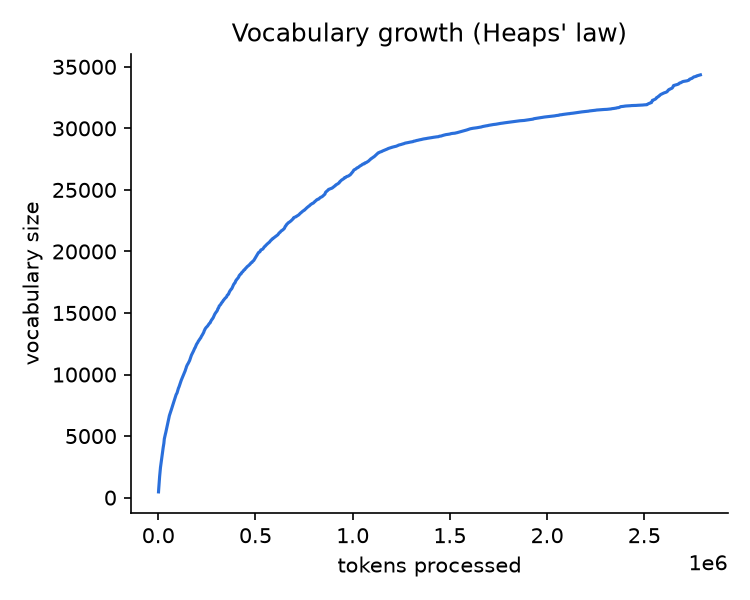
\includegraphics[width=\linewidth]{imgs/heaps.png}
  \caption{Vocabulary growth}
  \Description{Line chart of vocabulary size against tokens processed. The
  curve rises steeply to about 28000 terms at 1.1 million tokens, then grows
  slowly to about 32000 at 2.5 million tokens, and rises again to 34348 at
  the end.}
  \label{fig:heaps}
\end{figure}

\begin{figure*}[h]
  \centering
  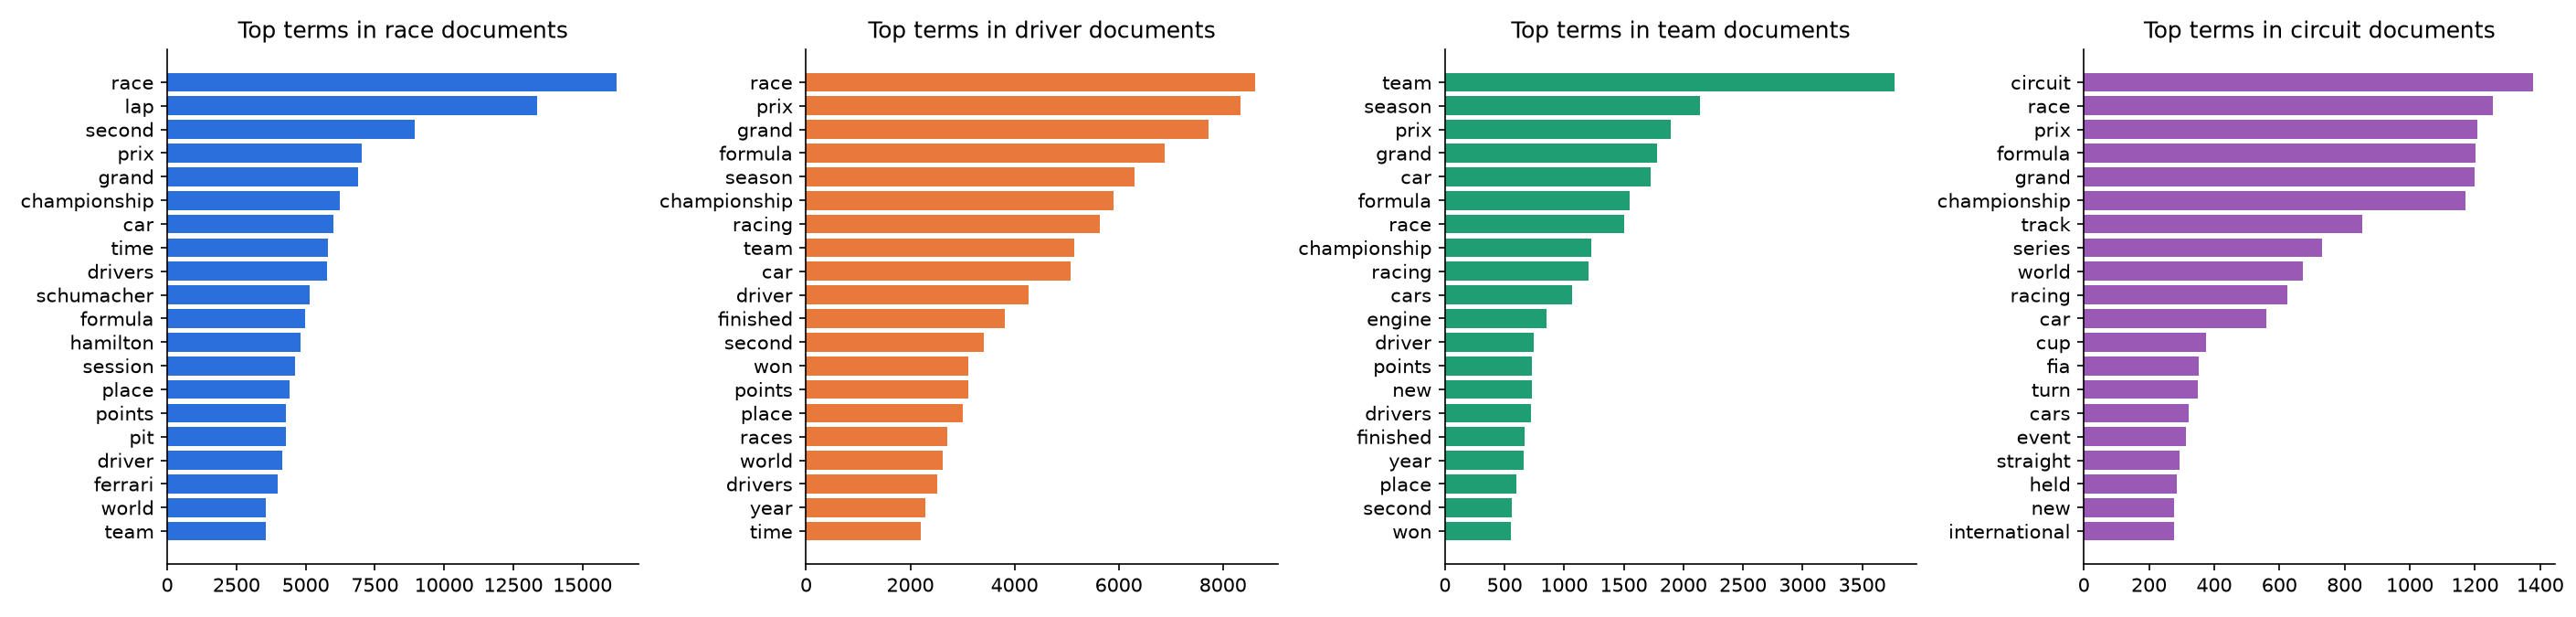
\includegraphics[width=\textwidth]{imgs/top_terms.png}
  \caption{Most frequent terms per document type, without stopwords}
  \Description{Four horizontal bar charts with the most frequent terms of
  race, driver, team and circuit documents. Race is led by ``race'' and
  ``lap''; driver by ``race'' and ``prix''; team by ``team'' and ``season'';
  circuit by ``circuit'' and ``race''.}
  \label{fig:topterms}
\end{figure*}

\begin{figure}[h]
  \centering
  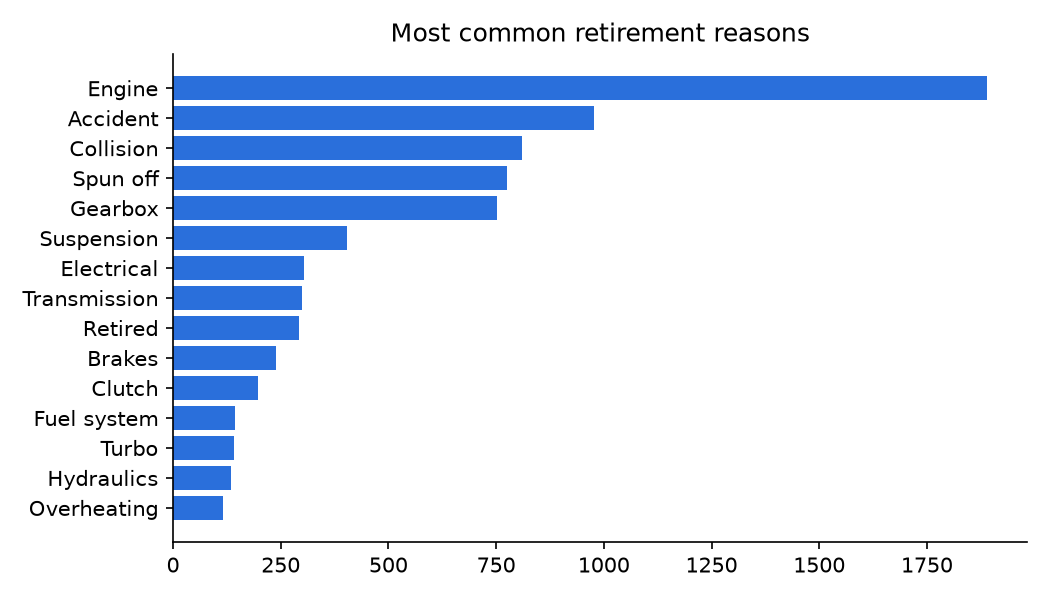
\includegraphics[width=\linewidth]{imgs/retirement_reasons.png}
  \caption{Most common retirement reasons}
  \Description{Horizontal bar chart of retirement reasons. Engine is the
  most common with 1889 cases, followed by accident, collision, spun off and
  gearbox.}
  \label{fig:retirements}
\end{figure}

\begin{figure}[h]
  \centering
  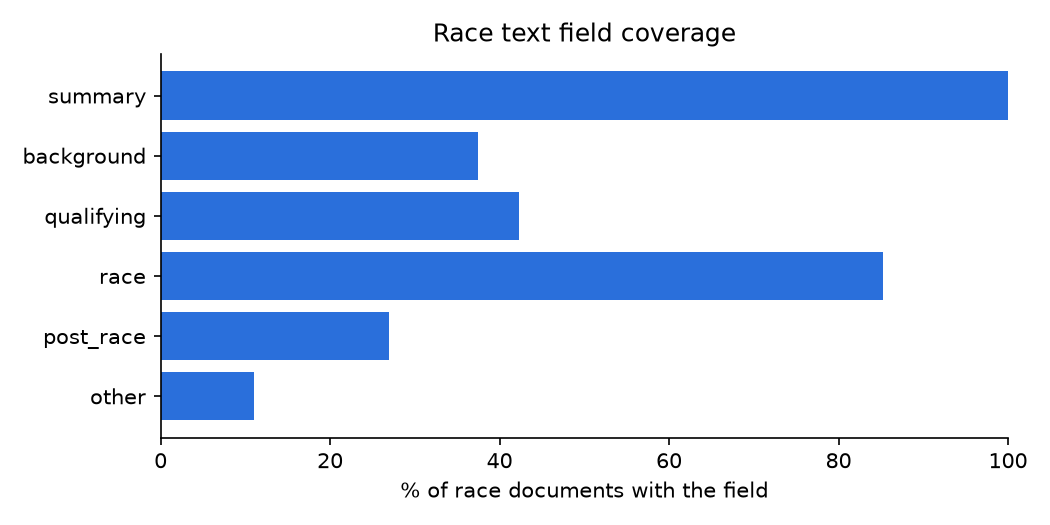
\includegraphics[width=\linewidth]{imgs/race_field_coverage.png}
  \caption{Share of race documents with each text field}
  \Description{Bar chart of the percentage of race documents with each text
  field: summary 100\%, race 85\%, qualifying 42\%, background 38\%,
  post-race 27\% and other 11\%.}
  \label{fig:coverage}
\end{figure}

\begin{figure}[h]
  \centering
  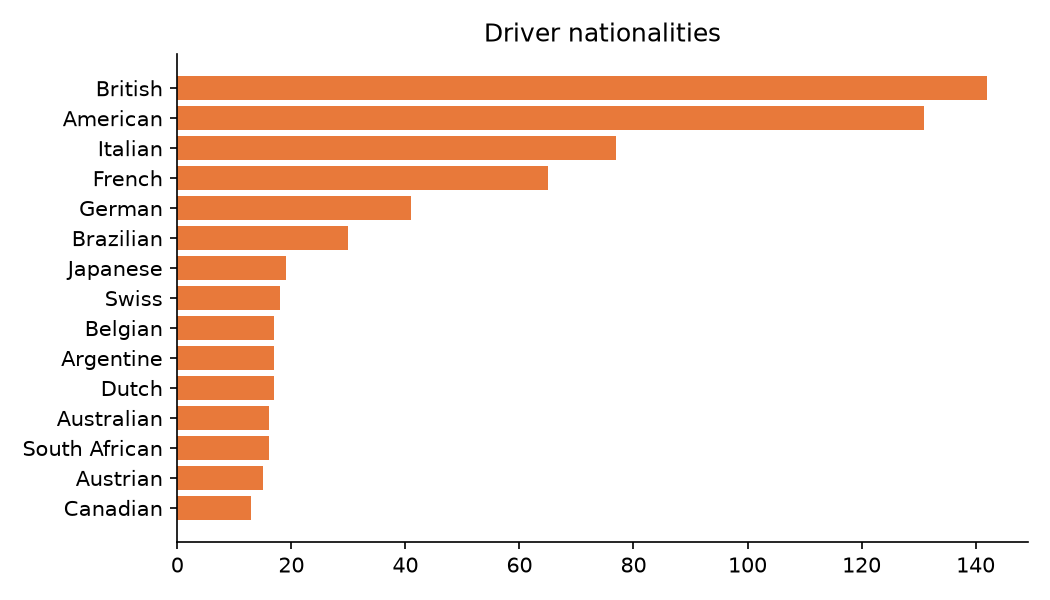
\includegraphics[width=\linewidth]{imgs/driver_nationalities.png}
  \caption{Driver nationalities}
  \Description{Horizontal bar chart of driver nationalities. British (142)
  and American (131) are the largest groups, followed by Italian, French and
  German.}
  \label{fig:nationalities}
\end{figure}

\begin{figure}[h]
  \centering
  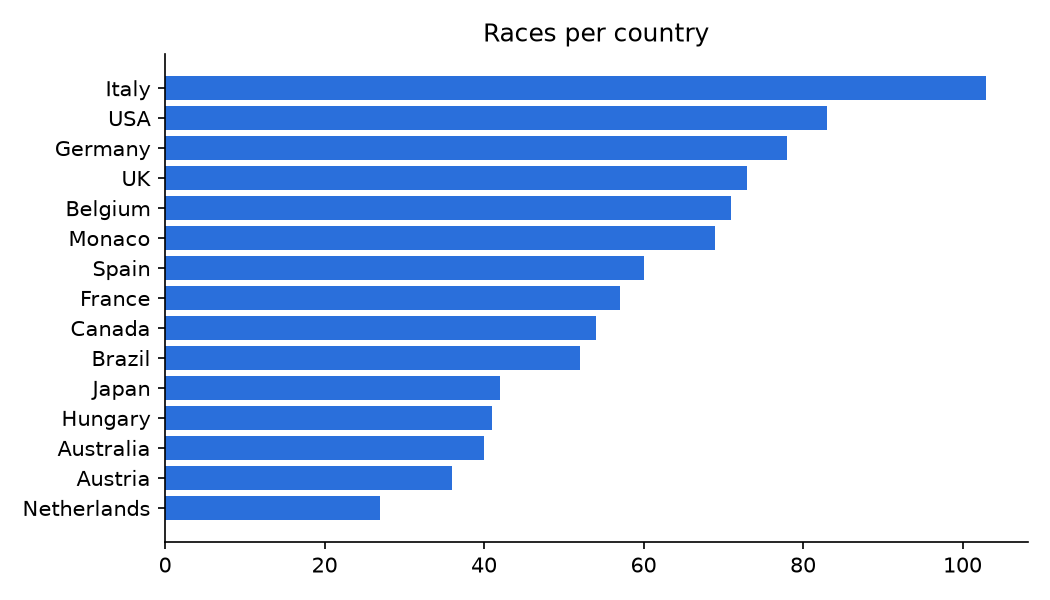
\includegraphics[width=\linewidth]{imgs/race_countries.png}
  \caption{Races per country}
  \Description{Horizontal bar chart of the number of races per country.
  Italy has the most with 103, followed by the USA, Germany, the United
  Kingdom, Belgium and Monaco.}
  \label{fig:countries}
\end{figure}

\section{Use of Generative AI}
Following the course policy, we declare that Claude Code (Anthropic) was
used during this milestone. It was used to help write and debug the code of
the data pipeline, to set up the \LaTeX{} template, and to draft and revise
parts of the text of this report from our notes, the project README and the
statistics produced by the pipeline. All the generated content was reviewed
by the group, and the numbers in the report were checked against the
output of the pipeline. The main prompts used were:
\begin{itemize}
  % TODO: substituir/completar com os prompts reais usados no código
  \item ``Write a script that downloads the Wikipedia articles linked in
  Jolpica in batches and resolves disambiguation pages.''
  \item ``What are the UML multiplicities between driver and team?''
  \item ``Write the Data Preparation section of the report based on the
  README, following the structure of the example report.''
  \item ``Write the remaining sections of the report with references.''
  \item ``Reduce the report to 4 pages and cover the required topics.''
\end{itemize}

\end{document}
